%%%%%%%%%%%%%%%%%%%%%%%%%%%%%%%%%%%%%%%%%%%%%%%%%%%%%%%%%%%%%%%%%%%%%%%%%%%%%%%
%%%%%%%%%%%%%%%%%%%%%%%%%%%%%%%%%%%%%%%%%%%%%%%%%%%%%%%%%%%%%%%%%%%%%%%%%%%%%%%
%%%%%%%%%%%%%%%%%%%%%%%%%%%%%%%%%%%%%%%%%%%%%%%%%%%%%%%%%%%%%%%%%%%%%%%%%%%%%%%
%%%%%%%%%%%%%%%%%%%%%%%%%%%%%%%%%%%%%%%%%%%%%%%%%%%%%%%%%%%%%%%%%%%%%%%%%%%%%%%
\chapter{Introduction}
\label{ch:intro}
%%%%%%%%%%%%%%%%%%%%%%%%%%%%%%%%%%%%%%%%%%%%%%%%%%%%%%%%%%%%%%%%%%%%%%%%%%%%%%%
%%%%%%%%%%%%%%%%%%%%%%%%%%%%%%%%%%%%%%%%%%%%%%%%%%%%%%%%%%%%%%%%%%%%%%%%%%%%%%%
%%%%%%%%%%%%%%%%%%%%%%%%%%%%%%%%%%%%%%%%%%%%%%%%%%%%%%%%%%%%%%%%%%%%%%%%%%%%%%%
%%%%%%%%%%%%%%%%%%%%%%%%%%%%%%%%%%%%%%%%%%%%%%%%%%%%%%%%%%%%%%%%%%%%%%%%%%%%%%%

A social insect society is formed by thousands of individuals, which continuously move and interact with each other inside a dark nest. 
Honey bees are organized in colonies, which form a complex and dynamical system.
Observing individual honey bees and their interactions with each other is, therefore, vital for understanding collective behavior and the organization of tasks within the colony.

Within the BeesBook project of the Biorobotics Lab of Freie Universität Berlin~\textcite{wario2015automatic} developed technologies to automatically track all individuals of a honey bee (Apis mellifera) colony, that are inside the honeycomb.
Shortly after hatching, each bee is marked on their thorax by using circular 12-bit tags (figure~\ref{fig:markers}) and then added to the observation colony. Four cameras observe the comb over a period of nine weeks, by capturing approximately three frames per second. An image analysis pipeline evaluates each frame automatically. The resulting data set contains, for each frame, the exact position of each detected bee on the honeycomb, and its age.

\begin{figure}[b]
	\centering
	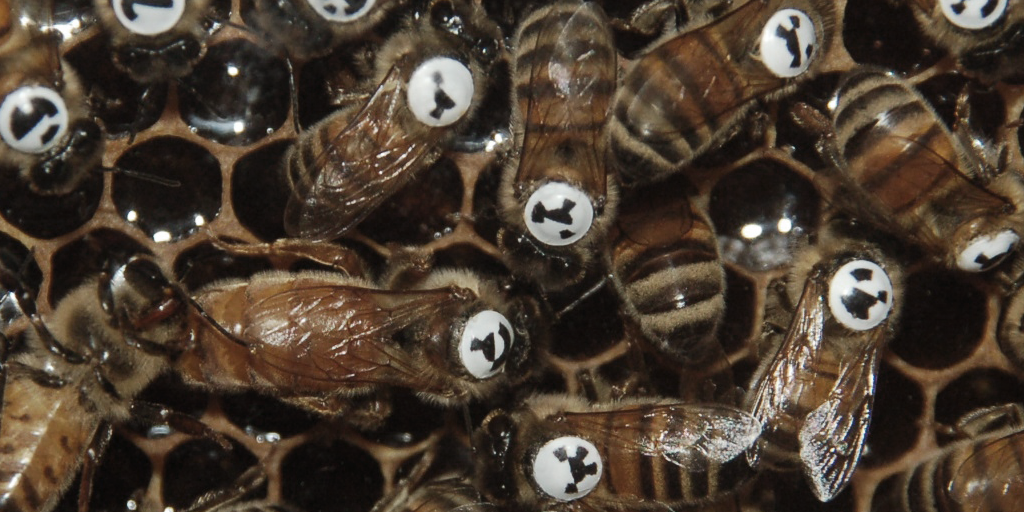
\includegraphics[width=1.0\textwidth]{Figures/markers}
	\caption{Tagged bees inside the observation hive.}
	\label{fig:markers}
\end{figure}

In this thesis, worker-worker interaction networks, based on spatial proximity, are derived from the described data set. Each node in the network is a bee, and a link between two nodes results if two bees are located close to each other over a specified period.
The networks are time-aggregated, which means one network represents the data of multiple frames.
After extracting the temporal networks, social network analysis methods are applied to determine the characteristics of the resulting networks and its communities.


%%%%%%%%%%%%%%%%%%%%%%%%%%%%%%%%%%%%%%%%%%%%%%%%%%%%%%%%%%%%%%%%%%%%%%%%%%%%%%%
%%%%%%%%%%%%%%%%%%%%%%%%%%%%%%%%%%%%%%%%%%%%%%%%%%%%%%%%%%%%%%%%%%%%%%%%%%%%%%%
\section{Motivation}
\label{sec:intro:motivation}
%%%%%%%%%%%%%%%%%%%%%%%%%%%%%%%%%%%%%%%%%%%%%%%%%%%%%%%%%%%%%%%%%%%%%%%%%%%%%%%
%%%%%%%%%%%%%%%%%%%%%%%%%%%%%%%%%%%%%%%%%%%%%%%%%%%%%%%%%%%%%%%%%%%%%%%%%%%%%%%
Colonies of social insects consist of a vast number of individuals.
The technique of manual insect tagging and tracking is widely applied in the behavioral sciences: First animals are marked using colored paint or numbered tags to distinguish individuals. Then, they are observed using a video recorder or by taking photos. The interaction data is obtained by repeatedly watching the video files and manually extracting events.
Consequently, labeling only a subset of the colonies individuals, a short observation period, a low number of frames, or limiting the observation to only a small area of the hive is very common.
Accordingly, most studies in the field of animal social network analysis, related to insects, analyzed only a reduced subset of a colonies' life. The majority of social insect interaction networks studies, due to previously technical limitations, aggregate temporal tracking data into a single static network~\cite[Chapter~15]{krause2014animal}.

Recently, automated tracking of insects has become technically feasible~\cite{wario2015automatic, crall2015beetag, fiala2005comparing}.
Using automated high resolution tracking data, which includes all individuals of the complete comb over an extended period allows for more advanced analysis focusing on temporal dynamics.
Therefore, automatic tracking allows shifting more towards the temporal and dynamic investigation.


%%%%%%%%%%%%%%%%%%%%%%%%%%%%%%%%%%%%%%%%%%%%%%%%%%%%%%%%%%%%%%%%%%%%%%%%%%%%%%%
%%%%%%%%%%%%%%%%%%%%%%%%%%%%%%%%%%%%%%%%%%%%%%%%%%%%%%%%%%%%%%%%%%%%%%%%%%%%%%%
\section{Research Goal and Method}
\label{sec:intro:goals}
%%%%%%%%%%%%%%%%%%%%%%%%%%%%%%%%%%%%%%%%%%%%%%%%%%%%%%%%%%%%%%%%%%%%%%%%%%%%%%%
%%%%%%%%%%%%%%%%%%%%%%%%%%%%%%%%%%%%%%%%%%%%%%%%%%%%%%%%%%%%%%%%%%%%%%%%%%%%%%%
The aim of this thesis is to investigate whether the provided data set of tracked honey bees is useful for creating worker-worker interaction networks using spatial proximity as an indicator for interactions between bees. Thus, I need to implement a pipeline to extract networks out of the given data set. Furthermore, I want to find out if the resulting networks are suitable for social network analysis.

I want to achieve my research goals by answering the following questions:

\begin{enumerate}
\item \emph{Is it possible to infer temporal networks with the provided honey bee tracking data?}\\
What challenges and limitations does the data set imply?
What pipeline parameters are necessary?
\item \emph{What kind of worker-worker interaction networks emerge and how are they structured?}\\
What is their topology?
What properties are characteristic and how do they differ from randomly generated networks?
\item \emph{Does the network display a meaningful community structure?}\\
How are the identified communities characterized?
Do they reflect already known colony behavior concerning age and spatial distribution?
\item \emph{How do these communities develop over time?}\\
Are they stable regarding their properties?
How do members move between communities?
\end{enumerate}


This work is meant to be the foundation to answer further more specific biological research questions using a network science approach to study the complex system of honey bee colonies and their collective behavior.

The methodology of this work consists of two parts, described in detail in Chapter~\ref{ch:approach}. The first part deals with the approach to infer and define spatial proximity networks using the given tracking data of honey bees. It serves as a prerequisite for analyzing the resulting networks concerning its network properties, communities and its development in the second part. 


\section{Outline}
This thesis is organized as follows. Chapter~\ref{ch:bg} gives a short introduction into social network analysis (SNA) and defines network measures, terms, and algorithms used throughout this work.
In chapter~\ref{ch:relatedwork}, a brief summary of the current state of research concerning social insect networks, temporal networks and community detection in animal social networks is given.
Chapter~\ref{ch:approach} describes my research approach in general and how the pipeline infers networks out of the given dataset, what steps are needed and what parameters it uses.
Also, I explain and justify what decisions I took during the network analyses and community detection process.
Chapter~\ref{ch:results} reports the results of the network analysis and the characteristics of the extracted communities.
Finally, in chapter~\ref{ch:conclusion} I explore the results, discuss limitations and conclude with directions for future work.